\chapter{输入/输出系统}\label{CO07}

\section{外部设备、显示存储与缓冲}\label{CO07-peripherals}

I/O硬件包括设备、接口/控制器及连接通路；软件包括驱动与上层管理程序。输入设备将外界信息采样编码，输出设备将编码转换成显示、声音或纸面记录，外存提供持久保存。

\par\smallskip
{\fontsize{9.3}{12}\selectfont\setlength{\tabcolsep}{2.5pt}\setlength{\LTleft}{0pt}\setlength{\LTright}{0pt}
\begin{longtable}{@{}>{\raggedright\arraybackslash}p{\dimexpr0.39353\linewidth-2\tabcolsep\relax}>{\raggedright\arraybackslash}p{\dimexpr0.60647\linewidth-2\tabcolsep\relax}@{}}
\toprule
设备 & 基本机制或参数 \\

\midrule\endfirsthead\toprule
设备 & 基本机制或参数 \\

\midrule\endhead\bottomrule\endfoot
键盘、鼠标 & 按键扫描编码，位移和按键形成报告 \\

扫描仪、摄像设备 & 光学信息采样编码 \\

显示器 & 屏幕尺寸、分辨率、每像素位数、刷新频率 \\

针式打印机 & 撞针经色带成像，可用于多联复写 \\

喷墨打印机 & 喷墨滴成像 \\

激光打印机 & 感光鼓成像、转印、定影 \\

\end{longtable}}
\par\smallskip

分辨率\(W\times H\)、每像素\(b\)位、刷新率\(f\)时，无压缩有效像素量：

\[
Q_{\mathrm{frame}}=\frac{WHb}{8}\ \mathrm B,\qquad
R_{\mathrm{pixel}}=\frac{WHbf}{8}\ \mathrm{B/s}.
\]

双缓冲容量为两帧，实际输出率按刷新频率计算。字模库存每种字符点阵，帧缓冲存当前画面像素；消隐、编码、包头与压缩按题设计入。1920\ensuremath{\times}1080、24位、60帧/s：单帧6220800 B，双缓冲12441600 B，有效速率373248000 B/s。

接口缓冲吸收瞬时速率差；持续输入高于长期消耗能力时，有限缓冲终会填满。

\section{I/O 接口、端口、编址与通道}\label{CO07-ports}

接口连接系统总线与设备，承担设备选择、地址识别、命令译码、数据缓冲、状态记录、串并转换、速度匹配，以及中断/DMA请求。端口是CPU可访问的接口寄存器或地址位置，一个接口通常包含多个端口。

\par\smallskip
{\fontsize{9.3}{12}\selectfont\setlength{\tabcolsep}{2.5pt}\setlength{\LTleft}{0pt}\setlength{\LTright}{0pt}
\begin{longtable}{@{}>{\raggedright\arraybackslash}p{\dimexpr0.34833\linewidth-2\tabcolsep\relax}>{\raggedright\arraybackslash}p{\dimexpr0.65167\linewidth-2\tabcolsep\relax}@{}}
\toprule
端口 & 内容与操作 \\

\midrule\endfirsthead\toprule
端口 & 内容与操作 \\

\midrule\endhead\bottomrule\endfoot
数据 & 读已接收数据、写待发送数据 \\

状态 & 读就绪、忙、错误等状态 \\

控制 & 写启动、复位、工作方式等命令 \\

\end{longtable}}
\par\smallskip

状态读与控制写可共享地址并由读写方向区分。端口地址定位接口位置，扇区地址定位设备内部数据。命令字、状态字、中断类型号均可经数据线传送；读写等控制线规定事务性质。

\par\medskip\Needspace{4\baselineskip}\noindent\hypertarget{CO07-E01}{}\label{CO07-E01}\textbf{例 7-1}\par\nobreak\smallskip

下列选项中，在I/O总线的数据线上传输的信息包括（　）。

I. I/O接口中的命令字　II. I/O接口中的状态字　III. 中断类型号

A. 仅 I、II　 B. 仅 I、III　 C. 仅 II、III　 D. I、II、III

\par\smallskip
\begin{wideblock}
{\fontsize{9.3}{12}\selectfont\setlength{\tabcolsep}{2.5pt}\setlength{\LTleft}{0pt}\setlength{\LTright}{0pt}
\begin{longtable}{@{}>{\raggedright\arraybackslash}p{\dimexpr0.31514\linewidth-2\tabcolsep\relax}>{\raggedright\arraybackslash}p{\dimexpr0.40787\linewidth-2\tabcolsep\relax}>{\raggedright\arraybackslash}p{\dimexpr0.27699\linewidth-2\tabcolsep\relax}@{}}
\toprule
编址 & 地址空间 & 访问方式 \\

\midrule\endfirsthead\toprule
编址 & 地址空间 & 访问方式 \\

\midrule\endhead\bottomrule\endfoot
统一编址/存储器映射I/O & 与主存共用；译码须区分内存和设备区域 & 普通访存指令 \\

独立编址 & 单独I/O空间；同数值可各对应内存和端口 & 通常用专门I/O指令 \\

\end{longtable}}
\end{wideblock}
\par\smallskip

接口与设备交换数据、命令和状态；接口向CPU提出中断请求。通道为执行通道程序的专用I/O处理部件，CPU启动后由其组织系列设备操作；通道指令由通道执行，I/O指令由CPU执行。DMA主要搬运设定数据块，通道可承担更完整控制组织。

\section{程序查询与服务期限}\label{CO07-polling}

查询流程：设置命令、地址与数量\ensuremath{\to}检查状态\ensuremath{\to}就绪后CPU读/写数据端口\ensuremath{\to}更新地址和计数\ensuremath{\to}完成或继续。忙等查询持续检查，等待及搬运均占CPU；定时查询在两次检查间可运行其他程序。

设设备速率\(R\) B/s、缓冲/每次交换\(q\) B，持续到达且每次取走一缓冲时：

\[
\Delta t_{\mathrm{buffer}}=\frac qR,\qquad
\lambda=\frac Rq\ \text{次/s},\qquad
U_{\mathrm{CPU}}=\lambda t_{\mathrm{service}}.
\]

查询与取数必须在缓冲覆盖前完成；单缓冲的服务间隔至多为\(q/R\)，还须将服务时长、相位及最长延迟纳入期限。已给每次服务\(c\)个周期、主频\(f\)时，\(U=\lambda c/f\)；已给\(I\)条指令时，\(c=I\times\mathrm{CPI}\)。

\par\medskip\Needspace{4\baselineskip}\noindent\hypertarget{CO07-E02}{}\label{CO07-E02}\textbf{例 7-2}\par\nobreak\smallskip

某计算机处理器主频为50 MHz，采用定时查询方式控制设备A的I/O，查询程序运行一次所用的时钟周期数至少为500。在设备A工作期间，为保证数据不丢失，每秒需对其查询至少200次，则CPU用于设备A的I/O的时间占整个CPU时间的百分比至少是（　）。

A. 0.02\%　 B. 0.05\%　 C. 0.20\%　 D. 0.50\%

50 MHz、每次查询100周期：鼠标每秒30次占0.006\%；磁盘2 MiB/s、每次4 B需\(2^{19}\)次/s，占约104.86\%，说明该组织服务能力不足。查询开销已包含搬运时，搬运费用只计一次。

\section{中断响应、现场与返回}\label{CO07-service}

中断I/O流程：CPU启动设备\ensuremath{\to}执行其他程序\ensuremath{\to}设备/接口发请求并用触发器保留\ensuremath{\to}CPU在允许边界判定未屏蔽请求\ensuremath{\to}硬件响应\ensuremath{\to}服务程序搬运与处理\ensuremath{\to}恢复返回。请求产生、允许响应、开始处理及完成分别计时。

\par\smallskip
{\fontsize{9.3}{12}\selectfont\setlength{\tabcolsep}{2.5pt}\setlength{\LTleft}{0pt}\setlength{\LTright}{0pt}
\begin{longtable}{@{}>{\raggedright\arraybackslash}p{\dimexpr0.34004\linewidth-2\tabcolsep\relax}>{\raggedright\arraybackslash}p{\dimexpr0.65996\linewidth-2\tabcolsep\relax}@{}}
\toprule
环节 & 典型动作 \\

\midrule\endfirsthead\toprule
环节 & 典型动作 \\

\midrule\endhead\bottomrule\endfoot
硬件响应 & 暂时禁止相应中断、保存断点和规定状态、定位入口 \\

软件入口 & 保存将修改且须恢复的通用寄存器及旧屏蔽字 \\

服务主体 & 读写数据端口、处理事件、设置控制信息 \\

软件退出/返回 & 关中断、恢复现场与屏蔽字、按ISA规则恢复断点和状态 \\

\end{longtable}}
\par\smallskip

中断向量为定位入口的信息，向量地址为保存向量的位置，处理程序入口为代码地址，具体映射由实现规定。单重中断在处理期间关闭相应可屏蔽中断。多重中断在现场保护和屏蔽设置完成后开放允许的嵌套。

教材单重序列常写“保护现场\ensuremath{\to}事件处理\ensuremath{\to}恢复现场\ensuremath{\to}开中断\ensuremath{\to}中断返回”；实际ISA也可由返回指令原子恢复状态与允许位。非屏蔽中断的响应时点及保存规则仍由体系结构规定。

\section{中断判优、屏蔽字与嵌套}\label{CO07-priority}

响应优先级由硬件在当前未屏蔽请求中选谁先响应；处理优先级规定服务程序间谁可打断谁，通过屏蔽字组织。屏蔽改变可参与响应的集合，保留已经发生的请求记录。

按屏蔽位1=禁止、0=允许的约定，服务程序通常屏蔽本级及不允许打断它的源，只开放更高处理优先级。每层进入时保存旧屏蔽字，退出时恢复上一层状态。

\par\medskip\Needspace{4\baselineskip}\noindent\hypertarget{CO07-E03}{}\label{CO07-E03}\textbf{例 7-3}\par\nobreak\smallskip

有A、B、C三个请求源，硬件响应优先级A\textgreater B\textgreater C。屏蔽字按A、B、C排列，1表示屏蔽。要求处理优先级C\textgreater B\textgreater A，服务程序均在保存现场并设置屏蔽字后开中断。给出三者的屏蔽字，并追踪三请求同时待处理时的一次嵌套过程。

请求的到达时间、屏蔽状态、嵌套关系和服务时长共同决定开始及完成顺序。初始响应按硬件优先级，嵌套返回按栈顺序。

\par\medskip\Needspace{4\baselineskip}\noindent\hypertarget{CO07-E04}{}\label{CO07-E04}\textbf{例 7-4}\par\nobreak\smallskip

若某设备中断请求的响应和处理时间为100 ns，每400 ns发出一次中断请求，中断响应所允许的最长延迟时间为50 ns，则在该设备持续工作过程中，CPU用于该设备的I/O时间占整个CPU时间的百分比至少是（　）。

A. 12.5\%　 B. 25\%　 C. 37.5\%　 D. 50\%

允许响应的最长延迟为期限；CPU占用只计实际响应/服务执行时间。每400 ns请求一次、服务100 ns，CPU占25\%；允许延迟50 ns另作实时性约束。

\section{DMA 控制器、传送阶段与访存方式}\label{CO07-direct}

DMA由控制器在设备接口与主存之间直接传数据。典型组成：主存地址寄存器/计数器、传送长度计数器、数据缓冲寄存器、设备地址、请求触发器、控制/状态逻辑及完成中断机构。

\par\smallskip
{\fontsize{9.3}{12}\selectfont\setlength{\tabcolsep}{2.5pt}\setlength{\LTleft}{0pt}\setlength{\LTright}{0pt}
\begin{longtable}{@{}>{\raggedright\arraybackslash}p{\dimexpr0.27041\linewidth-2\tabcolsep\relax}>{\raggedright\arraybackslash}p{\dimexpr0.72959\linewidth-2\tabcolsep\relax}@{}}
\toprule
阶段 & 执行主体与动作 \\

\midrule\endfirsthead\toprule
阶段 & 执行主体与动作 \\

\midrule\endhead\bottomrule\endfoot
预处理 & CPU驱动设置方向、主存起址、设备、长度等参数并启动 \\

数据传送 & 设备准备→请求DMA→DMA申请总线→授权后传送→更新地址和计数 \\

后处理 & 块结束/出错通知CPU，软件检查结果、处理错误、唤醒后续工作 \\

\end{longtable}}
\par\smallskip

\begin{figure}
\centering
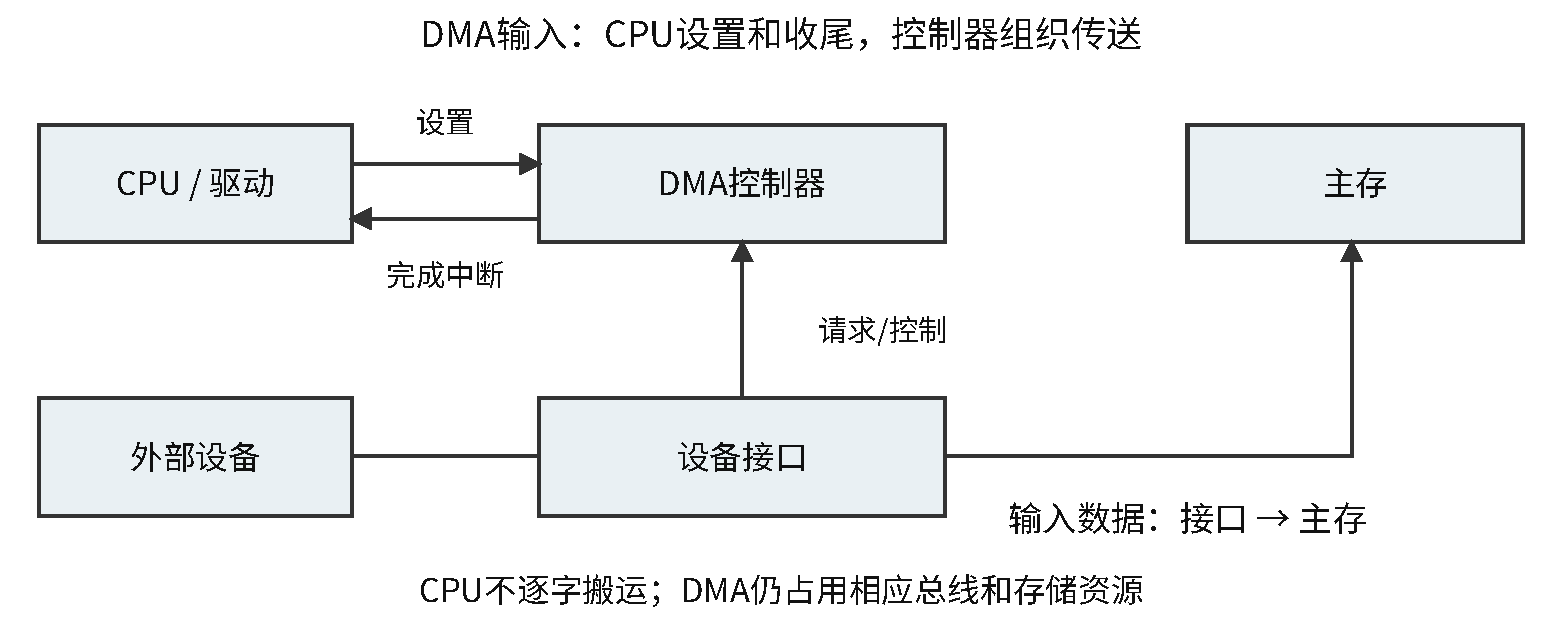
\includegraphics[width=\linewidth,height=108mm,keepaspectratio]{figures/CO_F12_dma_path.pdf}
\caption{CPU设置收尾，DMA在接口与主存间搬运}
\end{figure}

\par\smallskip
\begin{wideblock}
{\fontsize{9.3}{12}\selectfont\setlength{\tabcolsep}{2.5pt}\setlength{\LTleft}{0pt}\setlength{\LTright}{0pt}
\begin{longtable}{@{}>{\raggedright\arraybackslash}p{\dimexpr0.36695\linewidth-2\tabcolsep\relax}>{\raggedright\arraybackslash}p{\dimexpr0.63305\linewidth-2\tabcolsep\relax}@{}}
\toprule
DMA访存方式 & 占用与CPU行为 \\

\midrule\endfirsthead\toprule
DMA访存方式 & 占用与CPU行为 \\

\midrule\endhead\bottomrule\endfoot
停止CPU访存/成组传送 & 集中占用相关总线，期间CPU所需同资源访存受阻 \\

周期挪用 & 准备好一个/若干单位后借用存储周期，通常让已开始CPU访存先完成 \\

交替访存 & CPU与DMA按固定时隙分配，减少重复仲裁，需组织时序 \\

\end{longtable}}
\end{wideblock}
\par\smallskip

DMA占用共享资源时，CPU可在可用寄存器、Cache或其他独立资源上继续；停顿由实际资源需求决定。设备向DMA请求服务、DMA向系统申请总线为两层请求；DMA申请与请求CPU运行服务程序的中断分别判断。

\par\medskip\Needspace{4\baselineskip}\noindent\hypertarget{CO07-E05}{}\label{CO07-E05}\textbf{例 7-5}\par\nobreak\smallskip

若设备采用周期挪用DMA方式进行输入和输出，每次DMA传送的数据块大小为512字节，相应的I/O接口中有一个32位数据缓冲寄存器。对于数据输入过程，下列叙述中，错误的是（　）。

A. 每准备好32位数据，DMA控制器就发出一次总线请求\\
B. 相对于CPU，DMA控制器的总线使用权的优先级更高\\
C. 在整个数据块的传送过程中，CPU不可以访问主存储器\\
D. 数据块传送结束时，会产生``DMA传送结束''中断请求

\par\medskip\Needspace{4\baselineskip}\noindent\hypertarget{CO07-E06}{}\label{CO07-E06}\textbf{例 7-6}\par\nobreak\smallskip

下列关于DMA方式的叙述中，正确的是（　）。

I. DMA传送前由设备驱动程序设置传送参数\\
II. 数据传送前由DMA控制器请求总线使用权\\
III. 数据传送由DMA控制器直接控制总线完成\\
IV. DMA传送结束后的处理由中断服务程序完成

A. 仅 I、II　 B. 仅 I、III、IV　 C. 仅 II、III、IV　 D. I、II、III、IV

\section{查询、中断和 DMA 的开销预算}\label{CO07-budget}

设持续设备速率\(R\) B/s、每次数据交换\(q\) B、每块\(Q\) B、每次CPU服务\(t\) s、每块预后处理\(u\) s、每数据单位占总线\(b\) s：

\par\smallskip
{\fontsize{9.3}{12}\selectfont\setlength{\tabcolsep}{2.5pt}\setlength{\LTleft}{0pt}\setlength{\LTright}{0pt}
\begin{longtable}{@{}>{\raggedright\arraybackslash}p{\dimexpr0.32615\linewidth-2\tabcolsep\relax}>{\raggedright\arraybackslash}p{\dimexpr0.22948\linewidth-2\tabcolsep\relax}>{\raggedright\arraybackslash}p{\dimexpr0.44438\linewidth-2\tabcolsep\relax}@{}}
\toprule
量 & 计算式 & 条件 \\

\midrule\endfirsthead\toprule
量 & 计算式 & 条件 \\

\midrule\endhead\bottomrule\endfoot
查询/中断事件率 & \(R/q\) & 每次交换\(q\) B \\

查询/中断CPU比例 & \((R/q)t\) & 服务开销均已计入 \\

DMA完成事件率 & \(R/Q\) & 每块正常完成通知一次 \\

DMA软件CPU比例 & \((R/Q)u\) & 预处理及后处理按块计 \\

数据总线占用比例 & \((R/q)b\) & 单位传输不重叠，无额外未计开销 \\

\end{longtable}}
\par\smallskip

CPU预算与总线预算分别核算。比例大于1表示处理能力不足；平均CPU开销低于100\%后，还需核最长响应时间及缓冲期限。多级缓冲、批量中断、突发合并等条件改变事件粒度时，重新计数。

\par\smallskip
{\fontsize{9.3}{12}\selectfont\setlength{\tabcolsep}{2.5pt}\setlength{\LTleft}{0pt}\setlength{\LTright}{0pt}
\begin{longtable}{@{}>{\raggedright\arraybackslash}p{\dimexpr0.26317\linewidth-2\tabcolsep\relax}>{\raggedright\arraybackslash}p{\dimexpr0.45583\linewidth-2\tabcolsep\relax}>{\raggedright\arraybackslash}p{\dimexpr0.28099\linewidth-2\tabcolsep\relax}@{}}
\toprule
方式 & CPU介入 & 搬运主体 \\

\midrule\endfirsthead\toprule
方式 & CPU介入 & 搬运主体 \\

\midrule\endhead\bottomrule\endfoot
忙等查询 & 连续检查、逐单位搬运 & CPU指令 \\

定时查询 & 定期查询并搬运 & CPU指令 \\

中断I/O & 每请求响应后运行服务程序 & CPU指令 \\

DMA & 每块设置、完成后收尾 & DMA控制器 \\

\end{longtable}}
\par\smallskip

字符等低速设备常用查询/中断，大批量块传送常用DMA；选择依速率、粒度、缓冲和实现。512 B块、4 B缓冲为128次数据单位传送，正常完成通知一次。1024 B块则为256次4 B单位；总线事务数还取决于突发合并。

\par\medskip\Needspace{4\baselineskip}\noindent\hypertarget{CO07-E07}{}\label{CO07-E07}\textbf{例 7-7}\par\nobreak\smallskip

假定计算机的主频为500 MHz，CPI为4。现有设备A和B，其数据传输率分别为2 MB/s和40 MB/s，对应I/O接口中各有一个32位数据缓冲寄存器。请回答下列问题，要求给出计算过程。

（1）若设备A采用定时查询I/O方式，每次输入/输出都至少执行10条指令。设备A最多间隔多长时间查询一次才能不丢失数据？CPU用于设备A输入/输出的时间占CPU总时间的百分比至少是多少？

（2）在中断I/O方式下，若每次中断响应和中断处理的总时钟周期数至少为400，则设备B能否采用中断I/O方式？为什么？

（3）若设备B采用DMA方式，每次DMA传送的数据块大小为1000 B，CPU用于DMA预处理和后处理的总时钟周期数为500，则CPU用于设备B输入/输出的时间占CPU总时间的百分比最多是多少？

1 MB/s、每中断4 B、CPU开销2 μs，需50\% CPU；改为1024 B块、每块CPU开销20 μs，约1.953\%。两值均仅计软件执行，另核总线占用和服务期限。

\section{设备准备与服务执行的重叠时间}\label{CO07-overlap}

计算总历时先标出``启动下一单位''的时刻，CPU占用累计实际响应和服务指令。CPU 50 MHz、CPI=4；每字符设备准备0.5 ms=25000周期；每字符10线路位（1起始、7数据、1校验、1停止），持续设备最多2000字符/s。

若每中断响应10周期，服务20条指令，第15条启动下一字符，则后5条服务指令可与下一次准备重叠。稳定重复间隔为\(25000+10+15\times4=25070\)周期；1000字符约25070000周期，CPU实际用\(1000(10+20\times4)=90000\)周期。

若从首次启动准备计到第1000次服务完全结束，最后5条无后续准备可重叠，精确总历时为\(1000\times25070+5\times4=25070020\)周期。起止事件改变时相应补计启动和排空。
